\documentclass[border=45pt, multi, tikz]{standalone}
% based on https://github.com/HarisIqbal88/PlotNeuralNet
% tinytex::tlmgr_install("standalone")
% tinytex::tlmgr_install("import")
% tinytex::tlmgr_install("pgf")
% tinytex::tlmgr_install("positioning")
% tinytex::tlmgr_install("3d")
\usepackage{import}
\subimport{layers}{init}
\usetikzlibrary{positioning}
\usetikzlibrary{3d} %for including external image 

\def\ConvColor{rgb:yellow,5;red,2.5;white,5}
\def\PoolColor{rgb:yellow,5;red,15}
\def\FlatColor{rgb:blue,5;green,2.5;white,5}
\def\DenseColor{rgb:magenta,5;black,7}

\begin{document}
\begin{tikzpicture}

\tikzstyle{connection}=[black,every node/.style={sloped,allow upside down}]

%%%%%%%%%%%%%%%%%%%%%%%%%%%%%%%%%%%%%%%%%%%%%%%%%%%%%%%%%%%%%%%%%%%%%%%%%%%%%%%%%%%%%%%%

\node[canvas is zy plane at x=0] (temp) at (-3,0,0) {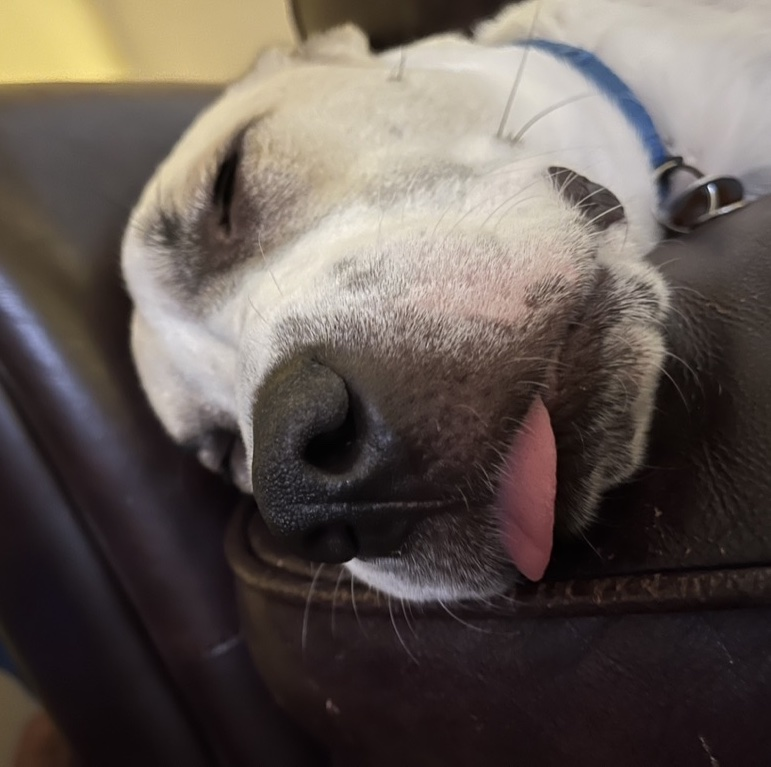
\includegraphics[width=8cm,height=8cm]{sleep.jpeg}};

\pic[shift={(.5,0,0)}] at (0,0,0) {Box={name=cr1,caption=\Large block 1,fill=\ConvColor,height=40,width={1, 1},depth=40}};

\pic[shift={(0,0,0)}] at (cr1-east) {Box={name=p1, fill=\PoolColor,opacity=0.5,height=20,width=1,depth=20}};


\pic[shift={(2.7,0,0)}] at (p1-east) {Box={name=cr2,caption=\Large block 2,fill=\ConvColor,height=20,width={2,2},depth=20}};

\pic[shift={(0,0,0)}] at (cr2-east) {Box={name=p2, fill=\PoolColor,opacity=0.5,height=9.9,width=2,depth=9.9}};


\pic[shift={(1.5,0,0)}] at (p2-east) {Box={name=cr3,caption=\Large block 3,fill=\ConvColor,height=9.9,width={4,4,4},depth=9.9}};

\pic[shift={(0,0,0)}] at (cr3-east) {Box={name=p3, fill=\PoolColor,opacity=0.5,height=4.8,width=4,depth=4.8}};


\pic[shift={(1.2,0,0)}] at (p3-east) {Box={name=cr4,caption=\Large block 4,fill=\ConvColor,height=4.8,width={8,8,8,8},depth=4.8}};

\pic[shift={(0,0,0)}] at (cr4-east) {Box={name=p4, fill=\PoolColor,opacity=0.5,height=2.4,width=8,depth=2.4}};


\pic[shift={(1.2,0,0)}] at (p4-east) {Box={name=cr5,caption=\Large block 5,fill=\ConvColor,height=2.4,width={8,8,8,8},depth=2.4}};

\pic[shift={(0,0,0)}] at (cr5-east) {Box={name=p5, fill=\PoolColor,opacity=0.5,height=1,width=8,depth=1}};



\pic[shift={(1.5,0,0)}] at (p5-east) {Box={name=flat,caption=\Large flatten,fill=\FlatColor,height=.75,width={.75},depth=55}};  % 1 / 150 * 8192

\pic[shift={(1.5,0,0)}] at (flat-east) {Box={name=dense,caption=\Large dense,fill=\DenseColor,height=.75,width={.75},depth=6.8}}; % 1 / 150 * 1024

\pic[shift={(1.5,0,0)}] at (dense-east) {Box={name=output,caption=\Large softmax,fill=\DenseColor,height=.75,width={.75},depth=1}};

%%%%%%%%%%%%%%%%%%%%%%%%%%%%%%%%%%%%%%%%%%%%%%%%%%%%%%%%%%%%%%%%%%%%%%%%%%%%%%%%%%%%%%%%

\draw [connection]  (p1-east)       -- node {\midarrow} (cr2-west);
\draw [connection]  (p2-east)       -- node {\midarrow} (cr3-west);
\draw [connection]  (p3-east)       -- node {\midarrow} (cr4-west);
\draw [connection]  (p4-east)       -- node {\midarrow} (cr5-west);
\draw [connection]  (p5-east)       -- node {\midarrow} (flat-west);
\draw [connection]  (flat-east)     -- node {\midarrow} (dense-west);
\draw [connection]  (dense-east)    -- node {\midarrow} (output-west);

%%%%%%%%%%%%%%%%%%%%%%%%%%%%%%%%%%%%%%%%%%%%%%%%%%%%%%%%%%%%%%%%%%%%%%%%%%%%%%%%%%%%%%%%


\end{tikzpicture}
\end{document}\grid
